% !TeX spellcheck = cs_CZ
{\tikzset{external/prefix={tikz/FYZI/}}
 \tikzset{external/figure name/.add={ch46_}{}}
%=========================== Kapitola: Rohatka se západkou ========================================
\chapter{Rohatka se západkou}\label{fyz:IchapXLVI}
\minitoc
  \section{Jak pracuje rohatka}\label{fyz:IchapXLVIsecI}
  \section{Rohatka jako stroj}\label{fyz:IchapXLVIsecII}
  \section{Vratnost v mechanice}\label{fyz:IchapXLVIsecIII}
  \section{Nevratnost}\label{fyz:IchapXLVIsecIV}
  \section{Uspořádání a entropie}\label{fyz:IchapXLVIsecV}
  \section{Příklady a cvičení}\label{fyz:IchapXLVIsecVI}

    \begin{figure}[ht!] %\ref{fyz_fig461}
      \centering
      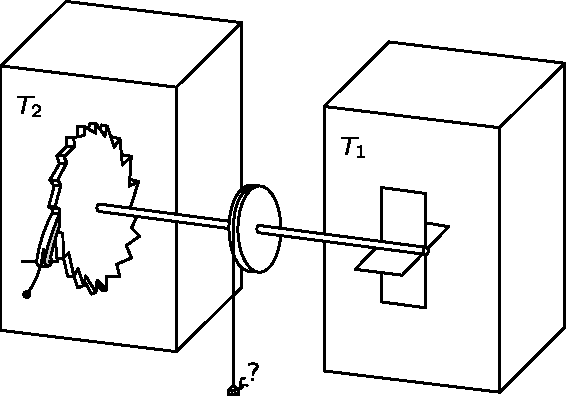
\includegraphics[width=0.7\linewidth]{fyz_fig461.pdf}
      \caption{ 
               (\cite[s.~707]{Feynman01})}
      \label{fyz_fig461}
    \end{figure}

    \begin{figure}[ht!] %\ref{fyz_fig462}
      \centering
      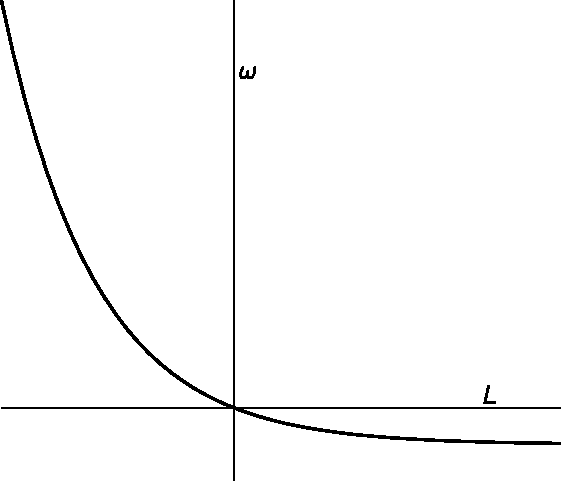
\includegraphics[width=0.7\linewidth]{fyz_fig462.pdf}
      \caption{ 
               (\cite[s.~707]{Feynman01})}
      \label{fyz_fig462}
    \end{figure}
} %tikzset
%---------------------------------------------------------------------------------------------------
\printbibliography[title={Seznam literatury}, heading=subbibliography]
\addcontentsline{toc}{section}{Seznam literatury}